\documentclass{article}
\usepackage{amssymb}
\usepackage[margin=0.8in]{geometry}
\usepackage{hyperref}
\usepackage{tikz}
\usepackage{caption}
\usepackage{tabularx}
\usepackage{subcaption}
\usepackage{bookmark}
\usepackage{listings}
\usepackage{paralist}
\usepackage{amsmath}
\usepackage{indentfirst}
\usepackage{graphicx}
\usepackage[toc,page]{appendix}
\graphicspath{{./images/}}
\newtheorem{theorem}{Theorem}[section]
\newtheorem{lemma}[theorem]{Lemma}
\newtheorem{proposition}[theorem]{Proposition}
\newtheorem{corollary}[theorem]{Corollary}
\newtheorem{definition}[theorem]{Definition}
\newtheorem{remark}[theorem]{Remark}
\newtheorem{property}[theorem]{Property}
\pagestyle{plain}

\usepackage{datetime}
\newdate{date}{22}{04}{2024}

\begin{document}
% \title{Math Meets Money}
\title{
 Math Meets Money \\ 
\begin{large} 
The intersection of combinatorics and finance for portfolio optimization and risk assessment
\end{large} }
\author{Blake Marterella}
\date{\displaydate{date}}

\maketitle

\section*{Abstract}

In this study we will explore the intersection of combinatorics and finance, specifically how graph theory can be used to optimize and assess risk in a stock portfolio. Using various theorem's and definitions in graph theory, we will analyze the composition of a portfolio to determine low risk, medium risk, and high risk holdings along with how the correlation between various stocks. Appliying mathematics to finance allows individuals to make more informed trades and mitigate risks by gaining insight to the mathematical signifigance of a stock price on any given day. A sample portfolio is introduced in this study, along with 4 years of historical stock data, but the concepts explored extend beyond this sample. The goal of this paper is to provide a theoretical framework for understanding portfolio optimization and risk assessment using advanced mathematical tools that can be applicable to any portfolio.

\tableofcontents

% [Introduction]
\section{Introduction}

\subsection{Brief History}

Mathematics has always been a powerful tool for humans to discover and describe seemingly complex patterns in the natural world. From the ancient days of arithemetic used to facilitate trade to the complex algorithms governing modern financial markets, mathematics has been an indispensable tool. The pivotal moment in the incorporation of mathematics into finance occured in 1654 when two great mathematicians, Blaise Pascal and Pierre de Fermat, developed probability theory to help predict the outcome of gambling [KD2010]. The ideas introduced in 1654 would evolve and help create the first automated trading system in 1949. Richard Donchian founded a commodity fund that used rule-based trading to execute trades based on moving averages in the market [LS2023]. These early pioneers set the stage for a methematical framework that would evolve into critical financial theories such as portfolio opimization, diversification, and risk management. In 2023, over 50\% of all trades in the US stock market were executed by algorithms [LS2023]. A critical tool in financal analysis is graph theory which can be used to represent the relationships between various stocks in a portfolio and help investors make more informed decisions.

% TODO revise the last two sentences for commas

\subsection{Interest}

The integration of combinatorics and finance, especially by the use of graph theory, is interesting for two main reasons. First, it provides a more comprehensive view to the correlations and diversification within a financial portfolio. Graph theory translates complex market dynamics into comprehensible, manageable models, allowing investors to visualize portfolio holdings in a new perspective and make informed decisions. Secondly, with the strategic application of graph theory, any individual's holdings can be optimized in such a way that investments remain not only sound but also resilient against market volatities. With the proper mathematical tools, any investor can have the power to make informed decisions just as large investment firms do.

\subsection{Motivation}

This study aims to democratize the complex mathematical strategies that find their place in financial markets so that more accessible knowledge and strategies are found for a more open audience. Though such advanced models have long been in use by large investment firms or hedge funds, it certainly would be of great value to put this kind of information in the hands of small investors. Through the examination of foundational concepts of graph theory and finance, this paper seeks to prepare the reader with the tools of understanding and engaging actively with their investment strategies.

The field of quantitative graph theory is rapidly expanding and encapsulating fields such as machine learning, graph algorithms, and quantitative analysis [MSFEYS2017]. This study serves as foundational and prerequisite knowledge to apply more complex analysis on financial data. By exploring the basics and providing  access to historical stock data, individuals can become powerful and successful independent traders.

% Let this flow into the definitions section

% [Main Section]
\section{Background}

\subsection{Data Collection}

For the purpose of this paper, I took the time to develop a custom API that allows me to quickly export historical data for a given stock [BM2024]. The API contains an endpoint that allows users to generate a CSV file for any given stock ticker and date range, providing 20 years of historical data. The csv file is loaded into a Pandas dataframe with the following fiels:

\begin{compactitem}
    \item \bf{Date} - The date of the stock price. 
    \item \bf{Open} - The opening price of the stock on that date.
    \item \bf{High} - The highest price the stock reached on that date.
    \item \bf{Low} - The lowest price the stock reached on that date.
    \item \bf{Close} - The closing price of the stock on that date.
    \item \bf{Volume} - The number of shares traded on that date.
\end{compactitem}

To enforce the concepts introduced in the paper, we will simulate a sample stock portfolio that contains 30 stocks from the DOW 30\footnote{The Dow Jones Industrial Average was selected because it is a relaitvely small list yet it is one of the most popular metrics to benchmark the stock exchange[DC2018]}. The API endpoint is used to pull a CSV file, hereby referred to as a dataset, for each stock in the portfolio that contains data from the past 4 years\footnote{The number, 4 years of DOW 30 historical data, was selected because it accounts for various financial markets}, along with the fields mentioned above.

\subsection{Data Processing}

Before continuing, it is important to understand how a graph can be constructed to represent using the datasets. Each stock within our portfolio will be represented as a vertex and the relationship between each stock will be represented as an edge. This edges can be drawn using many different relationships depending on what your graph is attempting to convey, such as: edges connecting companies in the same sector, edges connecting companies with similar market capitalization, etc. For the purpose of this study, each edge will be the correlation factor between stocks.

% Pearson Correlation Coefficent
\begin{definition}[Pearson Correlation Coefficent]
\[
r = \frac{\sum_{i=1}^n (X_i - \overline{X})(Y_i - \overline{Y})}{\sqrt{\sum_{i=1}^n (X_i - \overline{X})^2} \sqrt{\sum_{i=1}^n (Y_i - \overline{Y})^2}}
\]
\end{definition}


The Pearson Corelation Coefficient, denoted as $r$, is a measure of the linear relationship between two variables. In the context of this study, $r$ is the correlation between 2 stocks' closing price over a 4 year period. $X_i$ and $Y_i$ is the closing price of stock x and stock y on day $i$. $\overline{X}$ and $\overline{Y}$ is the average closing price of stock x and stock y over the 4 year period. In the formula above, the numerator calculates the covariance between 2 stocks and the deonominator uses product of stock x and stock y's standard deviation. The result is a number between -1 and 1, where -1 is a perfect negative linear relationship (as X increases, Y decreases), 1 is a perfect positive linear relationship (as X increases, Y increases), and 0 represents no linear relationship (there is no way X can predict Y)[ST2024]. 

Using the datasets in our portfolio, $r$ is calculated for each pair of stocks. The result is a correlation matrix. The table below shows a subsection of our correlation matrix using 4 stocks. Note that, the correlation for a stock with itself is always 1.0.

\begin{center}
\begin{tabularx}{0.8\textwidth}{ 
    | >{\centering\arraybackslash}X  
    | >{\centering\arraybackslash}X  
    | >{\centering\arraybackslash}X  
    | >{\centering\arraybackslash}X  
    | >{\centering\arraybackslash}X | } 
      \hline
       & \bf{AXP} & \bf{AMGN} & \bf{DIS} & \bf{DOW} \\ 
      \hline
      \bf{AXP} & 1 & 0.160404 & 0.553888 & 0.586814 \\ 
      \hline
      \bf{AMGN} & 0.160404 & 1 & 0.141811 & 0.192764 \\ 
      \hline
      \bf{DIS} & 0.553888 & 0.141811 & 1 & 0.463608 \\ 
      \hline
      \bf{DOW} & 0.586814 & 0.192764 & 0.463608 & 1 \\ 
      \hline
\end{tabularx}
\end{center}    

Figure 1 depicts a graph constructed with the correlation matrix that allows us to visualize the relationships between stocks in the portfolio using a color scale. Although the information presented is not usable, it provides a foundation for the application of graph theory in portfolio management.

\begin{figure}[h]
    \caption{Correlation Matrix Graph showing the relationships between 30 stocks in our sample portfolio}
    \centering
    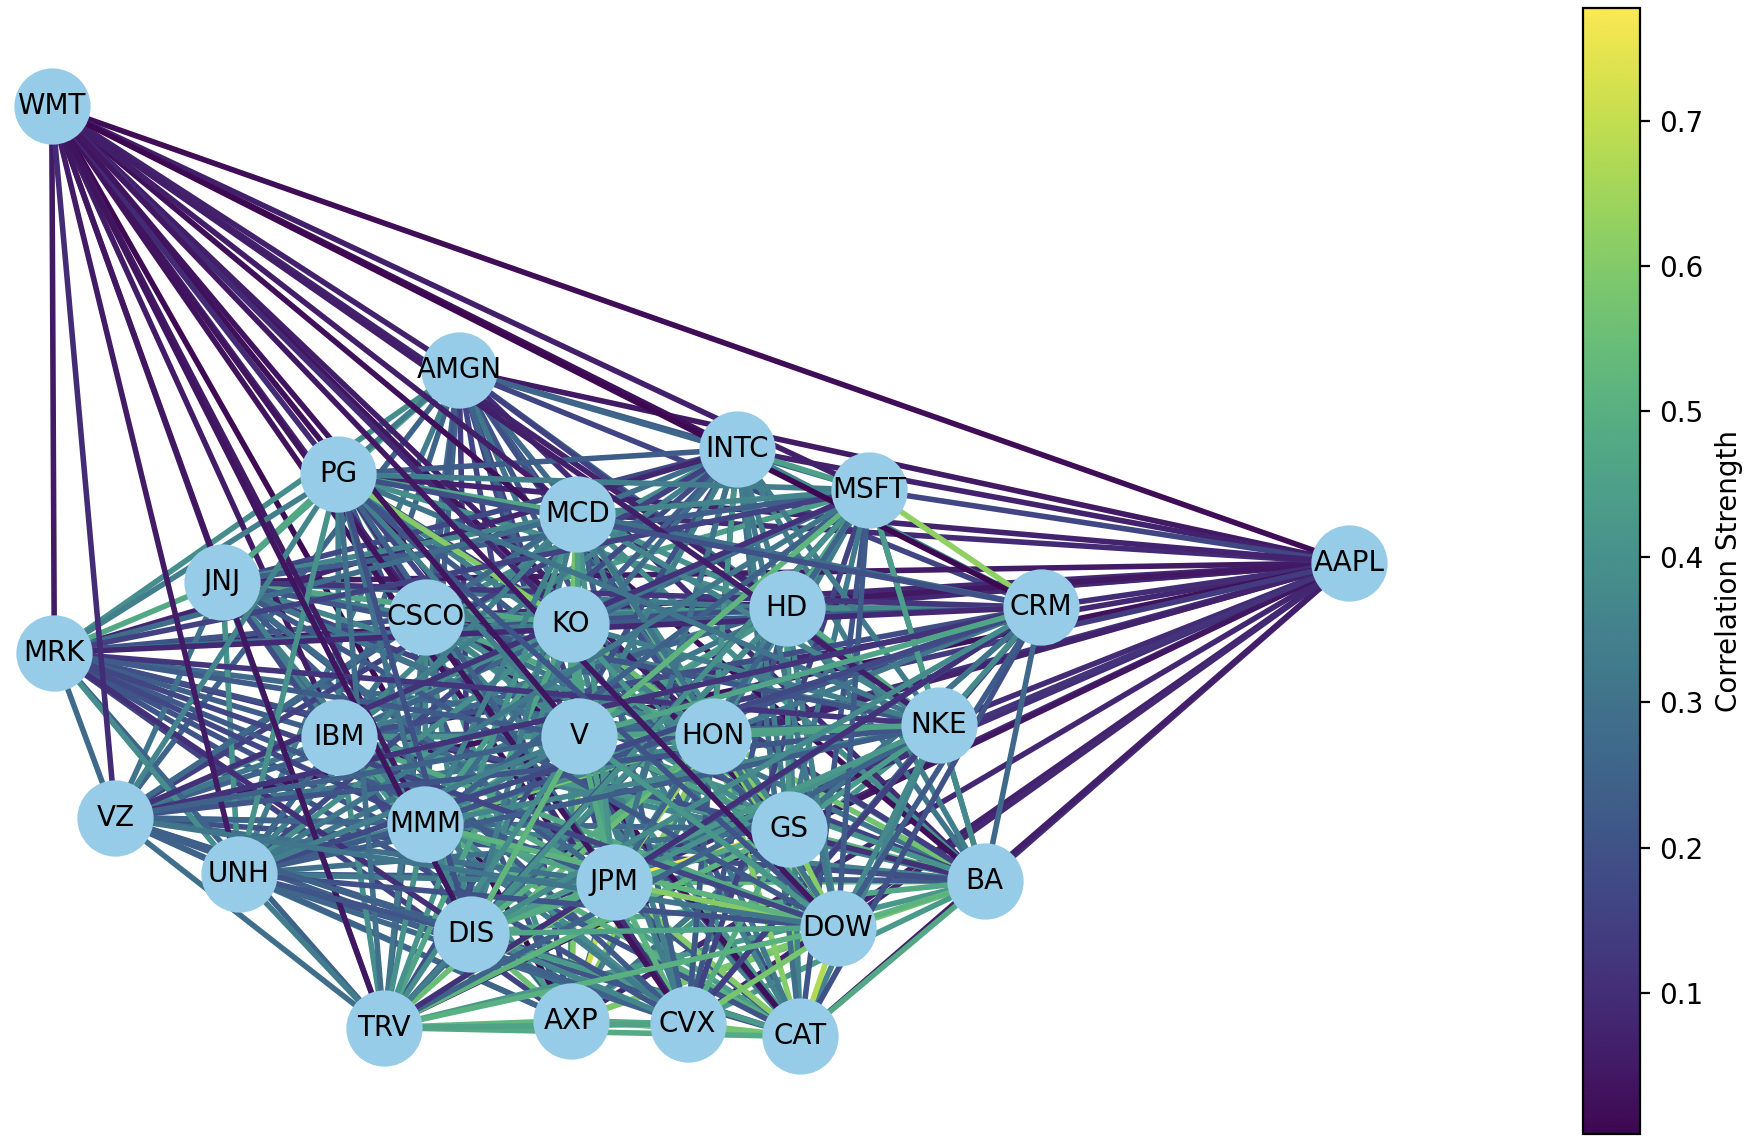
\includegraphics[width=0.5\textwidth]{correlation_matrix_graph.png}
\end{figure}    

The figure has 30 vertices and 435 total edges. The average number of degrees for each vertex is 29, meaning that the average stock is correlated with 29 other stocks in the portfolio. The maximum number of edges possible for an undirected graph without loops and 30 verties is $\binom {30}{2} = \frac{30 (30 - 1)}{2} = 435$ edges. Therefore the graph is dense because the number of edges is equal to the maximum number of edges possible. This is a sign that the portfolio is not well diversified and that there are many stocks that are highly correlated with each other. Additionally, the average correlation strength is 0.303. A diversified portfolio should have a low average correlation strength and a low number of edges. In the next section, we will explore how graph theory can be used to optimize and diversify a portfolio.


% % Greedy Coloring Algorithm

% \begin{definition}[Welsch-Powwell Algorithm]
% \end{definition}

% Go into detail about the coloring alogirthm



% Briefly define graph theory terms that will be used (vertices, edges, etc.). 


% Convert the concept of a portfolio from a spreadsheet to a graph with vertices and edges. This concept is the central point of the paper.



% [Main Section]
\section{Portfolio Optimization}

% Extremal Graph Theory
\begin{definition}[Extremal Graph Theorem] Let $G$ be a graph with $n$ vertices and $m$ edges. Then, if $G$ does not contain a subgraph isomorphic to $K_{r+1}$, the complete graph on $r+1$ vertices, then $m \leq \frac{r}{2}(n-1)$.
\end{definition}

Extremal Graph Thoerem is a powerful tool in portfolio optimiziation. The theorem can be particularly useful in preventing over-concentration of correlated assets, thus enhancing the robustness of the portfolio against market volatility. The theorem states that if a graph does not contain a subgraph isomorphic to $K_{r+1}$, then the number of edges in the graph is bounded by $\frac{r}{2}(n-1)$. In the context of a stock portfolio, avoiding a subgraph $K_{r+1}$ means ensuring that no group of $r+1$ stocks are all heavily correlated with each other. This helps in spreading out the investment risk by limiting the number of direct correlations any single stock has within the portfolio, thus achieving a higher degree of diversification. For example, a conservative portfolio may want to exclude any subset of 3 stocks from being mutually interconnected. In this case, $r = 3$ and $n = 30$ (since the portfolio contains 30 stocks). By applying the theorem, we can calculate the maximum number of edges allowed in the graph to maintain a diversified portfolio.

For further optimization, I only allowed an edge to be drawn in the graph if the correlation between two stocks was less than .2. This number was selected as it is less than the average correlations strength of the original graph show in Figure 1. Figure 2 shows a graph that does not contain cliques of size 3 or more and has a correlation threshold of .5. The resulting graph, shown in Figure 2, still has 30 nodes but the number of edges has been reduced to only 74. The average correlation strength for the graph is 0.08.

\begin{figure}[h]
    \caption{Extremal Graph Theory applied to the correlation matrix graph}
    \centering
    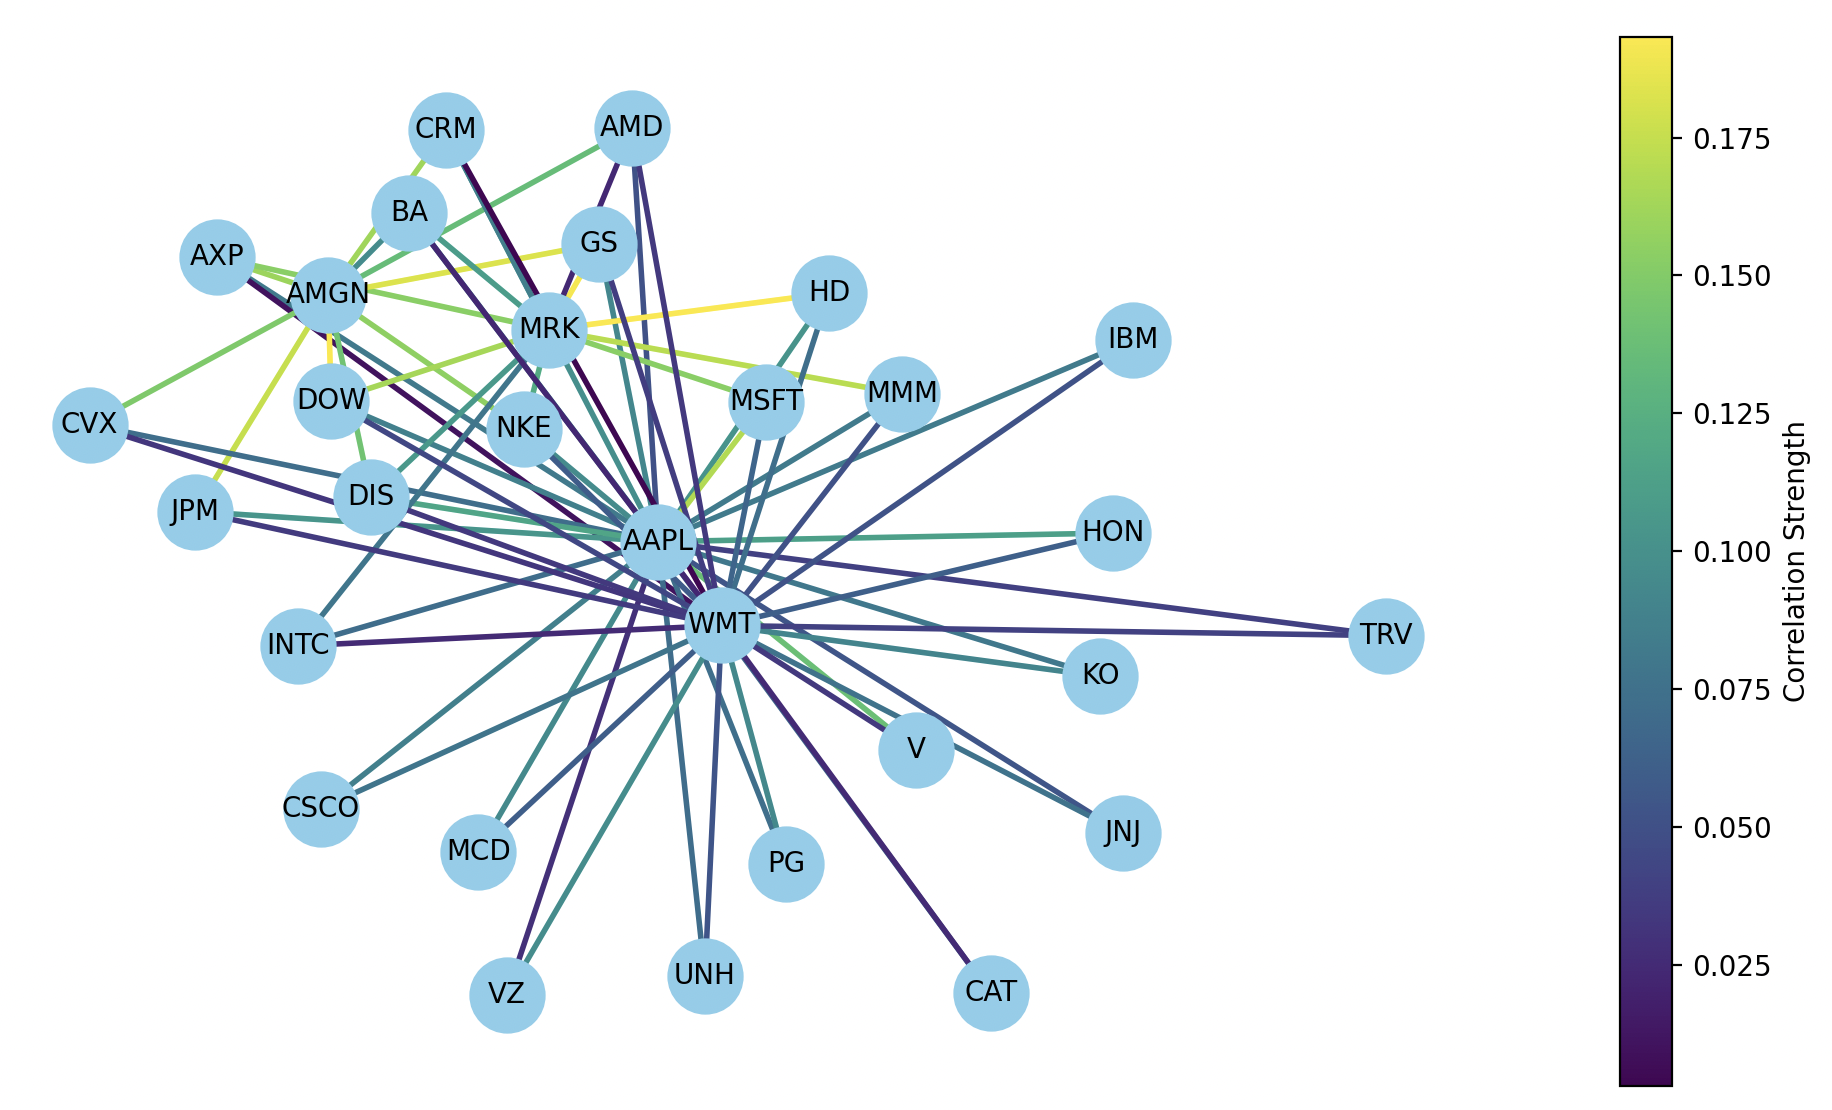
\includegraphics[width=0.7\textwidth]{extremal_graph_theory.png}
\end{figure}    



% [Main Section]
\section{Risk Management}
Coloring algorithms for risk assesment and management

\begin{itemize}
    \item Concept Introduction: Explain what graph coloring is and the significance of using different colors.
    \item Implementation: How coloring can be used to represent different levels of risk or different asset classes.
    \item Practical Example: A case study where coloring helps in decision-making about asset allocation or identifying over-concentrated sectors
\end{itemize}


% [Main Section]
\section{Holding Vizualization}

Correlation Graphs for Portfolio Holdings

\begin{itemize}
    \item Graph Construction: Discuss how to build a graph where vertices represent assets and edges represent correlations between returns.
    \item Analysis Techniques: Use threshold levels to add/remove edges or use weights to show the strength of correlations.
    \item Visualization: Include a section on how these graphs can visually represent portfolio diversification and the interconnections between assets.
\end{itemize}


\section{Conclusion}

\begin{itemize}
    \item Summary: Recap how graph theory enhances portfolio management.
    \item Future Directions: Suggest how further research could integrate other combinatorial techniques or advanced graph theory concepts.
    \item Open Problems: Pose any unresolved questions or potential for new research that your paper hints at.
\end{itemize}


\subsection{Future Development}


\bibliographystyle{alpha}
\begin{thebibliography}{99}
    % https://maa.org/sites/default/files/images/upload_library/46/NCTM/The-Pascal-Fermat-Correspondence.pdf
    \bibitem[KD2010]{Z}
    K. Devlin, \emph{The Pascal-Fermat Correspondance}, Mathematics Teacher, Vol. 103 \textbf{No. 8}, National Council of Teachers of Mathematics (2010), 580-582.
    % https://analyzingalpha.com/algorithmic-trading-history
    \bibitem[LS2023]{Z}
    L. Smigel, \emph{Algorithmic Trading History: A Breif Summary}, Analyzing Alpha (2023).
    % https://dl.acm.org/doi/abs/10.1016/j.ins.2017.08.009
    \bibitem[MSFEYS2017]{Z}
    M. Dehmer, S. Emmert-Streib, Y. Shi, \emph{Quantitative Graph Theory}, Information Sciences, Vol. 418 \textbf{Issue C}, Association for Computing Machinery Digital Library (2017).
    % https://www.scribbr.com/statistics/pearson-correlation-coefficient/
    \bibitem[ST2024]{Z}
    S. Turney, \emph{Pearson Correlation Coefficent}, Scribbr (2024).
    % https://evoq-eval.siam.org/Portals/0/Publications/SIURO/Volume%2010/Analysis_Equity_Markets_A_Graph_Theory_Approach.pdf
    % \bibitem[JAJCDBRGZC2017]{Z}
    % J. R. Abrams, J. C., D. B., R. G., Z. C., \emph{Analysis of Equity Markets: A Graph Theory Approach}, The University of Arizona, Department of Mathematics (2017).
    % https://www.fool.com/investing/2018/07/23/a-foolish-take-how-often-do-dow-stocks-get-replace.aspx
    \bibitem[DC2018]{Z}
    D. Caplinger, \emph{How Often Do Dow Stocks Get Replaced}, The Motley Fool (2018).
    % https://www.marterella.com/projects/stock-market-api
    \bibitem[BM2024]{Z}
    B. Marterella \emph{Stock Market API}, marterella.com (2024).
\end{thebibliography}

\clearpage

\begin{appendices}
    
\section{Code}

Note that the code below was modified from its original form to only show the relavant information. For example, function docstrings, input validation, etc. have been removed for brevity.

\subsection{Import Historical Stock Data}

\begin{lstlisting}[language=Python]
def get_stock_data(ticker, start=None, end=None):    
    url = f"{BASE_URL}historical-stock-data"
    params = {
        "symbol": ticker,
        "start": start,
        "end": end,
        "datatype": "json"
    }
    response = requests.get(url, params=params)

    if response.status_code == 200:
        data = response.json()  
        json_data = json.loads(data['data'])
    
        # Load the JSON data into a Pandas DataFrame
        df = pd.DataFrame(json_data) 
        df['date'] = pd.to_datetime(df['date'])
        
        # Ensure the directory exists and save CSV
        os.makedirs(os.path.dirname(path), exist_ok=True)
        df.to_csv(path, index=False)

        return df
    else:
        print("Failed to fetch data. Status code:", response.status_code)
        return None
\end{lstlisting}

\subsection{Import Historical Stock Data for Portfolio}

\begin{lstlisting}[language=Python]
def get_portfolio_data(tickers):
    portfolio_data = {}
    
    for ticker in tickers:
        start = datetime(year=2020, month=4, day=25).strftime('%Y-%m-%d')
        end = datetime(year=2024, month=4, day=24).strftime('%Y-%m-%d')
        ticker_df = get_stock_data(ticker, start=start, end=end)

        if ticker_df.empty:
            print(f"Failed to fetch data for {ticker}!")
            break
        else:
            portfolio_data[ticker] = ticker_df
    
    # Return dictionary of stock dat 
    return portfolio_data
\end{lstlisting}


\subsection{Get Pearson Correlation Coefficient}

\begin{lstlisting}[language=python]
def get_pearson_correlation_matrix(portfolio_data):
    returns = {name: df['close'].pct_change() for name, df in portfolio_data.items()}
    returns_df = pd.DataFrame(returns)

    return returns_df.corr(method='pearson')
\end{lstlisting}

\subsection{Display Graph}
This helper function makes displaying a graph using color mapped edges easier.

\begin{lstlisting}[language=python]
def draw_graph(G):
    pos = nx.spring_layout(G, k=0.2, scale=1)  # positions for all nodes

    # Generate edge colors based on weight
    weights = [G[u][v]['weight'] for u,v in G.edges()]
    edges = G.edges()
    edge_colors = plt.cm.viridis((np.array(weights) - min(weights)) / 
                                 (max(weights) - min(weights)))
    fig, ax = plt.subplots()

    # Drawing Nodes, Edges, and Labels
    nx.draw_networkx_nodes(G, pos, node_color='skyblue', node_size=700, ax=ax)
    nx.draw_networkx_edges(G, pos, edgelist=edges, edge_color=edge_colors, ax=ax)
    nx.draw_networkx_labels(G, pos, font_size=10, font_family='sans-serif', ax=ax)

    # Color bar settings
    sm = plt.cm.ScalarMappable(cmap=plt.cm.viridis, 
            norm=plt.Normalize(vmin=min(weights), vmax=max(weights)))
    sm.set_array([])
    cbar = plt.colorbar(sm, ax=ax, orientation='vertical')  
    cbar.set_label('Correlation Strength')

    plt.axis('off')
    plt.show()
\end{lstlisting}

\subsection{Draw Correlation Matrix Graph}

\begin{lstlisting}[language=python]
    def draw_correlation_matrix_graph(portfolio_data, corr_threshold=-1):
    correlation_matrix = get_pearson_correlation_matrix(portfolio_data)
    
    G = nx.Graph()
    for stock1 in correlation_matrix.columns:
        for stock2 in correlation_matrix.index:
            if stock1 != stock2 and correlation_matrix.loc[stock1, stock2] > corr_threshold:
                G.add_edge(stock1, stock2, weight=correlation_matrix.loc[stock1, stock2])
    
    draw_graph(G, image_name)
\end{lstlisting}

\clearpage

\subsection{Apply Extremal Graph Theory}

\begin{lstlisting}[language=python]
def apply_extremal_graph_theory(portfolio_data, corr_threshold=-1, max_clique_size=3):
    correlation_matrix = get_pearson_correlation_matrix(portfolio_data)
    G = nx.Graph()

    # Add edges based on the correlation threshold and avoiding cliques
    for stock1 in correlation_matrix.columns:
        for stock2 in correlation_matrix.index:
            if stock1 != stock2 and correlation_matrix.loc[stock1, stock2] < corr_threshold:
                # Tentatively add edge
                G.add_edge(stock1, stock2, weight=correlation_matrix.loc[stock1, stock2])

                # Check for cliques and remove the edge if it forms a forbidden clique
                if any(len(clique) >= max_clique_size for clique in nx.find_cliques(G)):
                    G.remove_edge(stock1, stock2)

    draw_graph(G, image_name)
\end{lstlisting}

\end{appendices}

\end{document}